%%%%%%%%%%%%%%%%%%%%%%%%%%%%%%%%%%%%%%%%%%%%%%%%%%%%%%%%%%%%%%%%%%%%%%%%%%%%%%%%
%2345678901234567890123456789012345678901234567890123456789012345678901234567890
%        1         2         3         4         5         6         7         8

\documentclass[letterpaper, 10 pt, conference]{ieeeconf}  % Comment this line out if you need a4paper

%\documentclass[a4paper, 10pt, conference]{ieeeconf}      % Use this line for a4 paper

\IEEEoverridecommandlockouts                              % This command is only needed if 
                                                          % you want to use the \thanks command

\overrideIEEEmargins                                      % Needed to meet printer requirements.

%In case you encounter the following error:
%Error 1010 The PDF file may be corrupt (unable to open PDF file) OR
%Error 1000 An error occurred while parsing a contents stream. Unable to analyze the PDF file.
%This is a known problem with pdfLaTeX conversion filter. The file cannot be opened with acrobat reader
%Please use one of the alternatives below to circumvent this error by uncommenting one or the other
%\pdfobjcompresslevel=0
%\pdfminorversion=4

% See the \addtolength command later in the file to balance the column lengths
% on the last page of the document

% The following packages can be found on http:\\www.ctan.org
%\usepackage{graphics} % for pdf, bitmapped graphics files
%\usepackage{epsfig} % for postscript graphics files
%\usepackage{mathptmx} % assumes new font selection scheme installed
%\usepackage{times} % assumes new font selection scheme installed
%\usepackage{amsmath} % assumes amsmath package installed
%\usepackage{amssymb}  % assumes amsmath package installed

\usepackage{cite}
\usepackage{amsmath}   % Required for align, matrices, and equation formatting
\usepackage{amssymb}   % Recommended for additional math symbols
\usepackage{bm}        % For bold symbols in equations
\usepackage{graphicx}  % Required if you include images
\usepackage{booktabs}   
\usepackage{caption}
\usepackage{url}
\usepackage{subcaption} 
\usepackage{afterpage}
\usepackage{float}  
\let\labelindent\relax
\usepackage{enumitem}

\title{\LARGE \bf
From Structural Design to Dynamics Modeling: 

Control-Oriented Development of a 3-RRR Parallel Ankle Rehabilitation Robot
}


% \author{Siyuan Zhang$^{1,}$\textsuperscript{*}, Yufei Zhang$^{1,2,}$\textsuperscript{*} and Junlin Lyu$^{1,}$\textsuperscript{*}% <-this % stops a space
% \thanks{*These author above contributed equally to this work.}% <-this % stops a space
% \thanks{$^{1}$Both in Mechanical Engineering,
%         Columbia University in the city of New York
%         {\tt\small}}%
% \thanks{$^{2}$Yufei Zhang is corresponding Author:
%         {\tt\small yz4917@columbia.edu}}%
% }
\author{Junlin Lyu$^{1,}$\textsuperscript{*}, Siyuan Zhang$^{1,}$\textsuperscript{*}, Yufei Zhang$^{1,}$\textsuperscript{*}, Sunil K. Agrawal$^{1, 2}$% <-this % stops a space
\thanks{*These authors contributed equally to this work.}% <-this % stops a space
\thanks{$^{1}$Department of Mechanical Engineering, 
        Columbia University in the City of New York.}%
\thanks{$^{2}$Prof.Sunil is the corresponding author: sa3077@columbia.edu}%
}

\begin{document}



\maketitle
\thispagestyle{empty}
\pagestyle{empty}


%%%%%%%%%%%%%%%%%%%%%%%%%%%%%%%%%%%%%%%%%%%%%%%%%%%%%%%%%%%%%%%%%%%%%%%%%%%%%%%%
\begin{abstract}

This paper presents the development of a wearable ankle rehabilitation robot based on a 3-RRR spherical parallel mechanism (SPM) to support multi-DOF recovery through pitch, roll, and yaw motions. The system features a compact, ergonomic structure designed for comfort, safety, and compatibility with ankle biomechanics. A complete design-to-dynamics pipeline has been implemented, including structural design, kinematic modeling for motion planning, and Lagrangian-based dynamic modeling for torque estimation and simulation analysis. Preliminary simulations verify stable joint coordination and smooth motion tracking under representative rehabilitation trajectories.

The control framework is currently being developed to enhance responsiveness across the workspace. Future work will focus on integrating personalized modeling and adaptive strategies to address kinematic singularities through model-based control.

This work establishes a foundational platform for intelligent, personalized ankle rehabilitation, enabling both static training and potential extension to gait-phase-timed assistance.

\end{abstract}


%%%%%%%%%%%%%%%%%%%%%%%%%%%%%%%%%%%%%%%%%%%%%%%%%%%%%%%%%%%%%%%%%%%%%%%%%%%%%%%%
\section{Introduction}

Ankle injuries are common among athletes, postoperative patients, and individuals with neurological impairments. Effective rehabilitation is critical for restoring mobility, strength, and proprioception. However, conventional rehabilitation devices often provide limited degrees of freedom (DOFs) \cite{dong2021state}, restricting natural joint movement and potentially prolonging recovery. Although robotic platforms with multi-DOF capabilities have been proposed, their bulky design and mechanical complexity frequently hinder clinical deployment and user compliance.

The human ankle can be biomechanically approximated as a spherical joint with three rotational DOFs: pitch (plantarflexion/dorsiflexion), roll (inversion/eversion), and yaw (internal/external rotation). To replicate this natural movement, we propose a 3-RRR spherical parallel manipulator (SPM) as the core of a wearable ankle rehabilitation robot. SPMs are known for their high stiffness, compact structure, and precise motion control, making them suitable for joint therapy applications. While the 3-RRR configuration has been extensively studied in robotics \cite{gosselin1989optimum}, finger rehabilitation \cite{he2021spindle}, and hip therapy \cite{sadeqi2017design}, its integration into wearable ankle rehabilitation remains largely unexplored.

This work establishes a complete design-to-control framework: from mechanical design and kinematic analysis to Lagrangian-based dynamic modeling and simulation-driven control development. The system is currently being validated through dynamic simulation, with control strategies under development to ensure smooth and stable actuation across the ankle’s workspace.

The remainder of this letter is organized as follows: Section II describes the mechanical design; Section III focuses on kinematic analysis for motion planning, and Section IV introduces the dynamic formulation for control integration; Section V discusses control simulation and validation; and Section VI concludes conclusion with future directions.

\section{Mechanism Design}

\subsection{Overview of the 3-RRR SPM}
A 3-RRR spherical parallel mechanism (SPM) consists of three identical limbs, each with two revolute (R) joints connecting a fixed base to a moving platform. This configuration enables compact, symmetric structures capable of generating three rotational degrees of freedom (DOFs) about a common center of rotation. While the 3-RRR architecture has been widely studied in robotics \cite{merlet2006parallel}, its application to wearable ankle rehabilitation remains limited.

\begin{figure}[h]
\centering
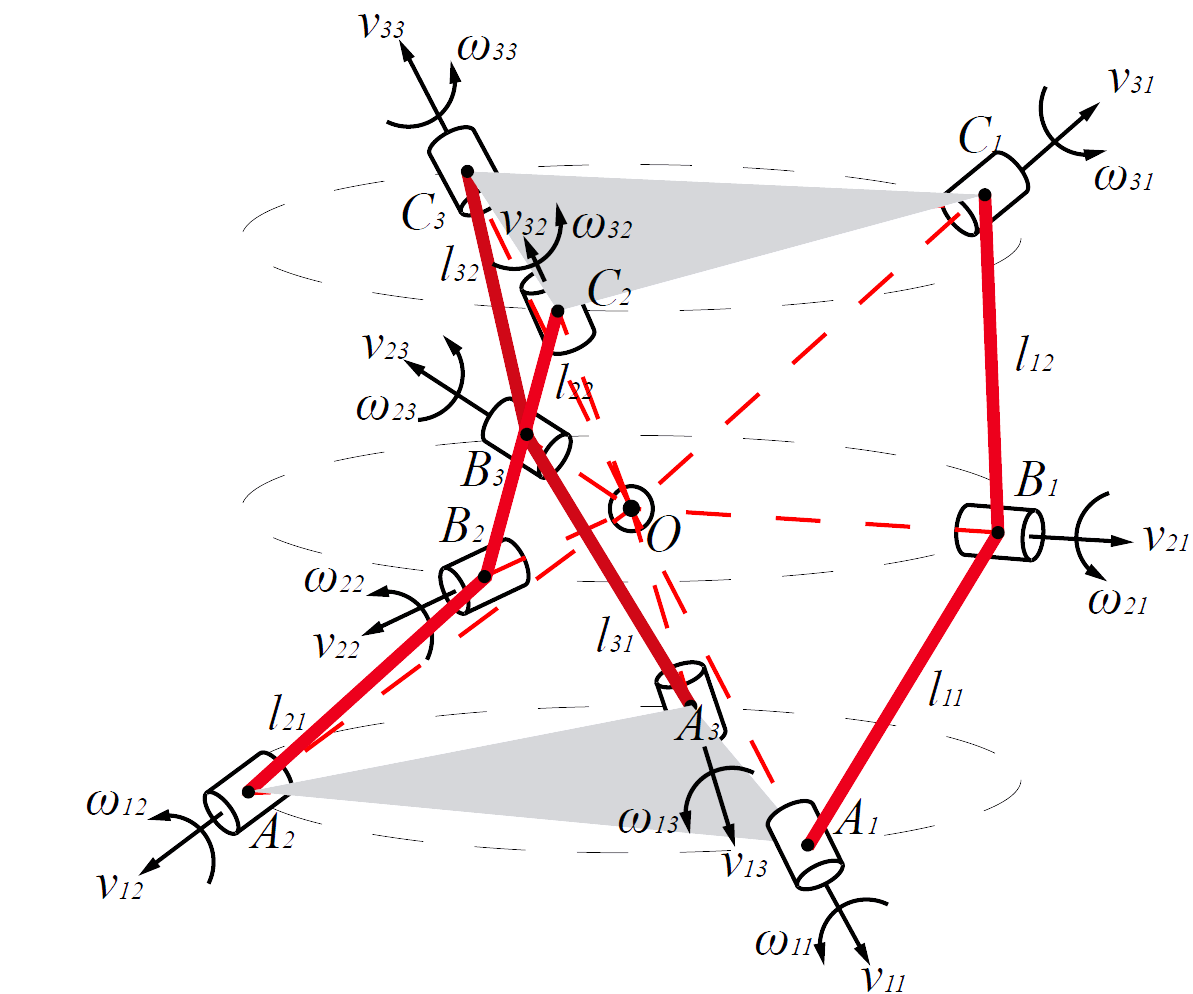
\includegraphics[width=0.67\linewidth]{SimplifiedModel.png}
\caption{Schematic geometry model of the 3-RRR mechanism.}
\label{fig:3rrr-model}
\end{figure}

As illustrated in Fig.~\ref{fig:3rrr-model}, the proposed design features a ring-shaped base and a footplate platform. By adjusting limb lengths and angular placements, the mechanism replicates pitch, roll, and yaw movements corresponding to dorsiflexion, inversion, and rotation of the ankle. The mechanism’s mobility is computed as 3, with 8 links and 9 revolute joints.

The wearable form factor introduces engineering constraints, but enables portable, multi-DOF rehabilitation. This makes the system suitable for both clinical use and athlete recovery scenarios where space efficiency and functional range are critical.

\subsection{Design Considerations}
This device is designed for direct lower limb attachment, promoting daily use and better patient compliance. A wearable form factor requires both mechanical and ergonomic considerations:

\subsubsection{Compact Base Ring}
Custom-fitted with adjustable straps for a secure, comfortable attachment.

\subsubsection{Non-Interference Mechanisms}
Low-profile limbs and joint housings minimize obstruction to nearby joints and ensure compatibility with footwear and braces.

\subsubsection{Device Modularity}
Interchangeable links and quick-release fasteners support adjustment across users and rehabilitation stages.

\begin{figure}[H]
    \centering
    \begin{subfigure}{0.15\textwidth}
        \centering
        
\includegraphics[width=\textwidth]{model.png}
        \caption{Rendered Model}
        \label{fig:fig1}
    \end{subfigure}
    \begin{subfigure}{0.15\textwidth}
        \centering
        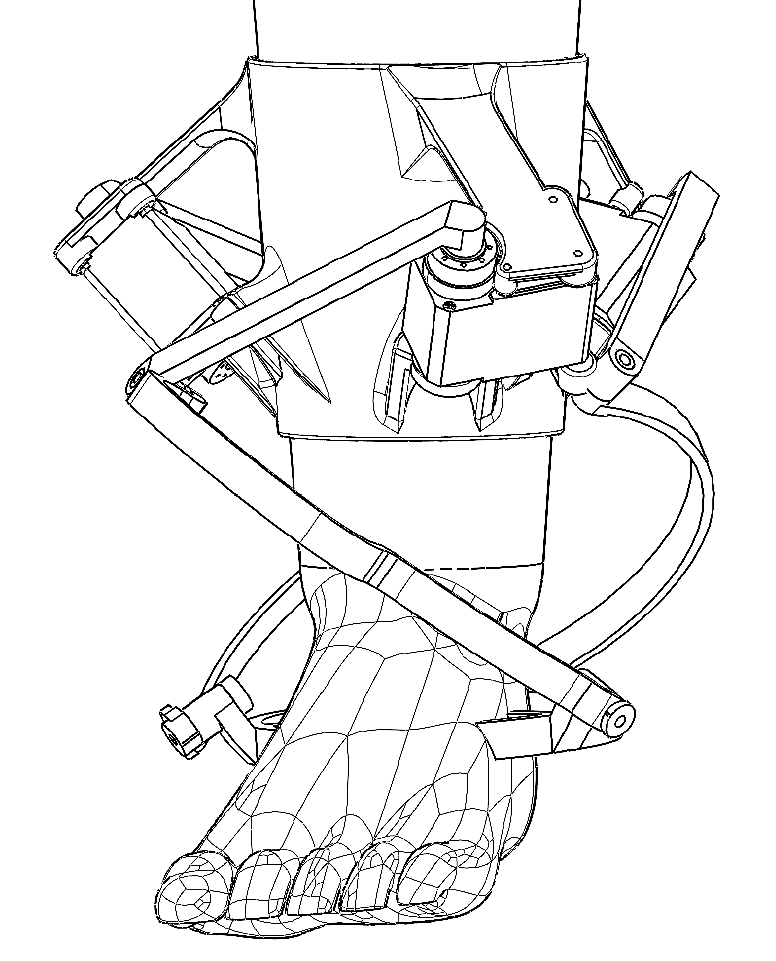
\includegraphics[width=\textwidth]{blackwhite.png}
        \caption{Line Drawing}
        \label{fig:fig2}
    \end{subfigure}
    \caption{SolidWorks CAD model}
    \label{fig:Solidworks Model}
\end{figure}  

\subsection{Detail Design}
To validate the design, a SolidWorks CAD model was created, highlighting the base ring, limbs, and footplate. The structure was optimized for workspace, compactness, and portability, balancing weight and strength to support user comfort and effective rehabilitation.

\begin{figure}[h]
    \centering
    \begin{subfigure}{0.15\textwidth}
        \centering
        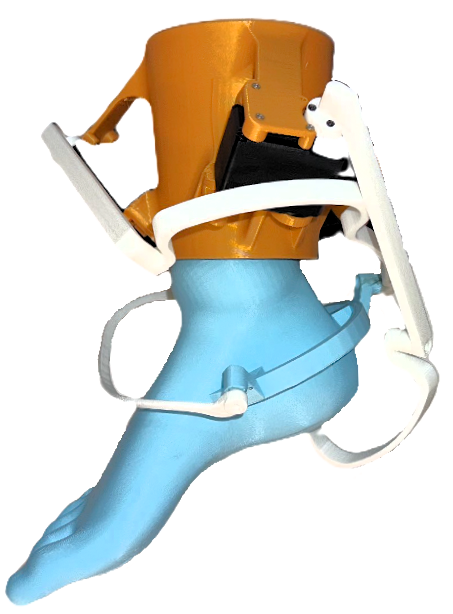
\includegraphics[width=\textwidth]{pitch.png}
        \caption{Pitch}
        \label{fig:fig1}
    \end{subfigure}
    \begin{subfigure}{0.15\textwidth}
        \centering
        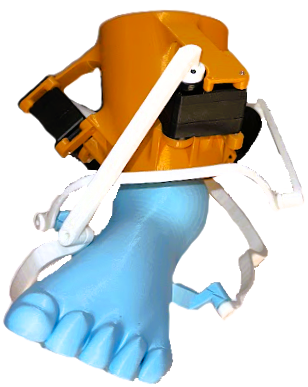
\includegraphics[width=\textwidth]{roll.png}
        \caption{Roll}
        \label{fig:fig2}
    \end{subfigure}
    \begin{subfigure}{0.16\textwidth}
        \centering
        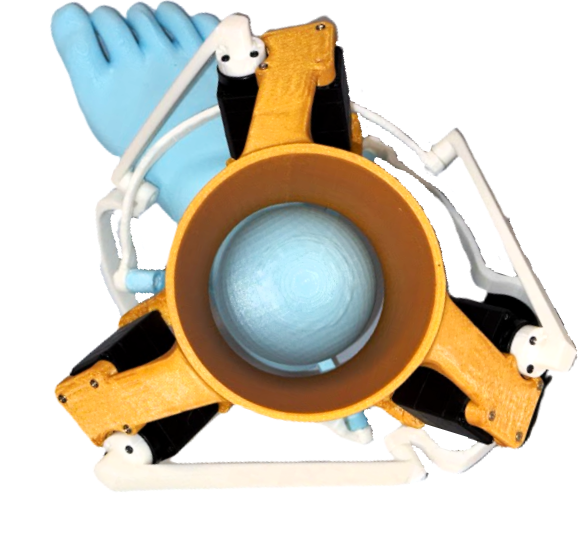
\includegraphics[width=\textwidth]{yaw.png}
        \caption{Yaw}
        \label{fig:fig3}        
    \end{subfigure}
    \caption{3D printed and view for the rehabilitation device.}
    \label{fig:combined2}
\end{figure}

A 3D-printed prototype was fabricated for physical validation. Fig.~\ref{fig:combined2} shows the assembled device, demonstrating structural fit and wearable integration.



\section{Kinematic Analysis}
\label{sec:kinematics}

This section establishes the mapping between the platform pose and individual joint motions. We first define all symbols, then compare coordinate representations, derive frame transformations, and finally present inverse, forward, and velocity kinematics. These results underpin the dynamic modeling in Section~\ref{sec:dynamics}.

\subsection{Geometry and Notation}
\label{sec:geometry}
Table~\ref{tab:geo} lists the key points and vectors for leg \(i\).

\begin{table}[h]
  \centering
  \caption{Points and vectors on leg \(i\).}
  \label{tab:geo}
  \begin{tabular}{@{}ll@{}}
    \toprule
    Symbol & Definition \\
    \midrule
    \(A_i\) & Actuated base joint \\
    \(B_i\) & Passive spherical joint \\
    \(C_i\) & Platform connection point \\
    \(P\)   & Platform center \\
    \(\mathbf r_i = B_i - P\) 
           & Vector \(P\to B_i\) \\
    \(\mathbf L_i = \tfrac{C_i - B_i}{\|C_i - B_i\|}\) 
           & Unit link direction \(B_i\to C_i\) \\
    \bottomrule
  \end{tabular}
\end{table}

% \subsection{Coordinate Representations}
% \label{sec:coords}
% To describe the 3‑DOF ankle motion, we adopt spherical coordinates \((R,\psi,\phi)\). 

% \begin{table}[h]
%   \centering
%   \caption{Spherical vs.\ Cartesian}
%   \label{tab:coords}
%   \renewcommand{\arraystretch}{1.1}
%   \begin{tabular}{@{}lcc@{}}
%     \toprule
%       & \textbf{Spherical} & \textbf{Cartesian} \\
%       & \((R,\psi,\phi)\)  & \((x,y,z)\)          \\
%     \midrule
%     \# vars          & 3          & 3           \\
%     FK               & direct     & nonlinear   \\
%     IK               & closed‑form& iterative   \\
%     Computational    & moderate   & low         \\
%     Data redundancy  & reduced    & higher      \\
%     \bottomrule
%   \end{tabular}
% \end{table}

\subsection{Frame Transformations}
\label{sec:frames}
A point \(C_{i0}\) in the platform frame is mapped to the base frame by
\[
  C_i = R(\alpha,\beta,\gamma)\,C_{i0}, 
  \quad
  R(\alpha,\beta,\gamma) = R_z(\alpha)\,R_y(\beta)\,R_x(\gamma).
\]
% Its Cartesian coordinates \((x,y,z)\) convert to spherical via
% \[
%   (x,y,z)
%   = \bigl(R\cos\psi\cos\phi,\;R\sin\psi\cos\phi,\;R\sin\phi\bigr),
% \]
% with \(\psi\) the azimuth about \(z\) and \(\phi\) the elevation from the \(xy\)-plane.

\subsection{Inverse Kinematics}
\label{sec:ik}
Given a desired pose \((R_P,\psi_{P},\phi_{P})\), each leg must satisfy
\[
  \|B_i - A_i\| = l_1, 
  \quad 
  \|C_i - B_i\| = l_2.
\]
Let
\[
  d = \|C_i - A_i\|,\;
  \lambda = \tfrac{l_1^2 - l_2^2 + d^2}{2d^2},\;
  \mu = \sqrt{l_1^2 - \lambda^2 d^2}.
\]
Then
\[
  B_i = A_i + \lambda(C_i - A_i)
       \pm \mu\,
       \frac{(C_i - A_i)\times N}{\|(C_i - A_i)\times N\|},
\]
and the active angle
\[
  \theta_i = \cos^{-1}\!\bigl(\tfrac{(B_i - A_i)\cdot u_i}{\|B_i - A_i\|}\bigr),
\]
with \(N\) a normal vector and \(u_i\) the joint‑axis direction.

\subsection{Forward Kinematics}
\label{sec:fk}
For known \(\theta_i\), the joint and platform positions follow
\[
  B_i = A_i + R_i(\theta_i)\,[l_1,0,0]^T,\quad
  C_i = B_i + R(\alpha,\beta,\gamma)\,[l_2,0,0]^T.
\]
Extracting \((\alpha,\beta,\gamma)\) from the resulting \(C_i\) completes the pose.

\subsection{Velocity Kinematics}
\label{sec:vel-kin}
Under pure rotation (\(\dot P=0\)), 
\[
  \mathbf v_{B_i} = \omega\times \mathbf r_i,
  \quad
  \dot q_i = \mathbf L_i^{T}(\omega\times \mathbf r_i).
\]
Stacking for \(i=1,2,3\) yields
\[
  \dot{\mathbf q} = J_r\,\omega,\quad
  J_r = 
  \begin{bmatrix}
    (r_1\times L_1)^T\\
    (r_2\times L_2)^T\\
    (r_3\times L_3)^T
  \end{bmatrix}.
\]
The Jacobian \(J_r\) relates joint rates to platform angular velocity; its conditioning will be critical in the dynamic control design.

% Section IV will use these kinematic mappings to derive the Lagrangian dynamics.


% Detailed Euler‑angle derivations are provided in the Appendix.


\section{Dynamics Modeling}
\label{sec:dynamics}

\subsection{Generalized Coordinates Definition}
Let the generalized coordinates be
\[
  \mathbf{q} = \begin{bmatrix}\theta_1\\\theta_2\\\theta_3\end{bmatrix},
\]
where \(\theta_i\) are the actuated revolute angles of the 3‑RRR spherical parallel mechanism.

\subsection{Energy Expressions}
\begin{enumerate}[label=\alph*)]
  \item \textbf{Kinetic Energy \(T\):}
    \begin{equation}
      T = \tfrac12\,\boldsymbol{\omega}^T I_P\,\boldsymbol{\omega}
          + \tfrac12\sum_{i=1}^3 I_{\ell,i}\,\dot\theta_i^2,
    \end{equation}
    where
    \begin{itemize}
      \item \(I_P\) is the inertia tensor of the moving platform.
      \item \(I_{\ell,i}\) is the moment of inertia of link \(i\) about its active joint.
    \end{itemize}

  \item \textbf{Potential Energy \(V\):}
    \begin{equation}
      V = 0,
    \end{equation}
    In this system, gravitational potential energy does not contribute to the rigid limbs, so the gravity term may be omitted:
    \begin{equation}
      G(\mathbf{q}) = 0.
    \end{equation}
\end{enumerate}

\subsection{Lagrangian and Equations of Motion}
Define the Lagrangian
\[
  L = T - V = T.
\]
Applying Lagrange’s equations,
\begin{equation}
  \frac{d}{dt}\Bigl(\frac{\partial L}{\partial\dot{\mathbf{q}}}\Bigr)
  -
  \frac{\partial L}{\partial \mathbf{q}}
  =
  \boldsymbol{\tau}.
\end{equation}
Collecting terms yields the rigid‑body equations
\begin{equation}
  M(\mathbf{q})\,\ddot{\mathbf{q}}
  + C(\mathbf{q},\dot{\mathbf{q}})\,\dot{\mathbf{q}}
  = \boldsymbol{\tau},
\end{equation}
where
\begin{align}
  M(\mathbf{q})
  &= J^+{}^{T}W^T I_P\,W\,J^+ \;+\; \mathrm{diag}(I_{\ell,1},I_{\ell,2},I_{\ell,3}),\\
  C_{jk}
  &= \tfrac12\sum_{i=1}^3
    \Bigl(
      \frac{\partial M_{jk}}{\partial \theta_i}
      + \frac{\partial M_{ji}}{\partial \theta_k}
      - \frac{\partial M_{ik}}{\partial \theta_j}
    \Bigr)\dot{\theta}_i.
\end{align}

These dynamics will be used in Section~\ref{sec:control} to design a model-based controller that compensates for inertial coupling and achieves precise, stable tracking across the workspace.  
\section{Control Design and Simulation Validation}
\label{sec:control}
To regulate the 3‑RRR SPM about its three rotational degrees of freedom (roll, pitch, yaw), we employ independent PID loops on each axis.  In order to investigate how \emph{compliance}—here, the effective “softness” introduced by lower feedback gains—affects the closed‑loop dynamics, we compare two tuning sets: an \emph{underdamped} response (low damping ratio) and a \emph{critically damped} (unit‑damped) response.

\subsection{PID Controller Structure}
Each axis is controlled by
% \[
%   \tau_i(t) = K_{p,i} e_i(t) + K_{d,i}\,\dot e_i(t) + K_{i,i}\int_0^t e_i(\sigma)\,d\sigma,
% \\
%   \quad
%   e_i = q_{i,\mathrm{ref}} - q_i,
% \]
\begin{align}
  \tau_i(t) &= K_{p,i}\,e_i(t) + K_{d,i}\,\dot{e}_i(t) \notag \\
            &\quad + K_{i,i} \int_0^t e_i(\sigma)\,d\sigma,
\end{align}
\[
  e_i = q_{i,\mathrm{ref}} - q_i,
\]

where \(i\in\{\mathrm{roll},\mathrm{pitch},\mathrm{yaw}\}\).  The same structure is used on all three axes, but gains are tuned to achieve the desired damping ratio.

\subsection{Gain Tuning and Compliance Effect}
To demonstrate the compliance effect, we selected:
\begin{itemize}
  \item \textbf{Underdamped case:} \(K_p = 20\), \(K_d = 0.5\), \(K_i = 1\).  
    The low derivative gain yields a damping ratio \(\zeta < 1\), producing oscillatory settling.
  \item \textbf{Critically damped case:} \(K_p = 50\), \(K_d = 2\), \(K_i = 5\).  
    These higher gains raise \(\zeta\approx1\), eliminating overshoot and oscillation.
\end{itemize}
Lower gains simulate a “softer” compliant behavior, where the platform freely oscillates before converging; higher gains stiffen the response.

\begin{figure}[h]
  \centering
  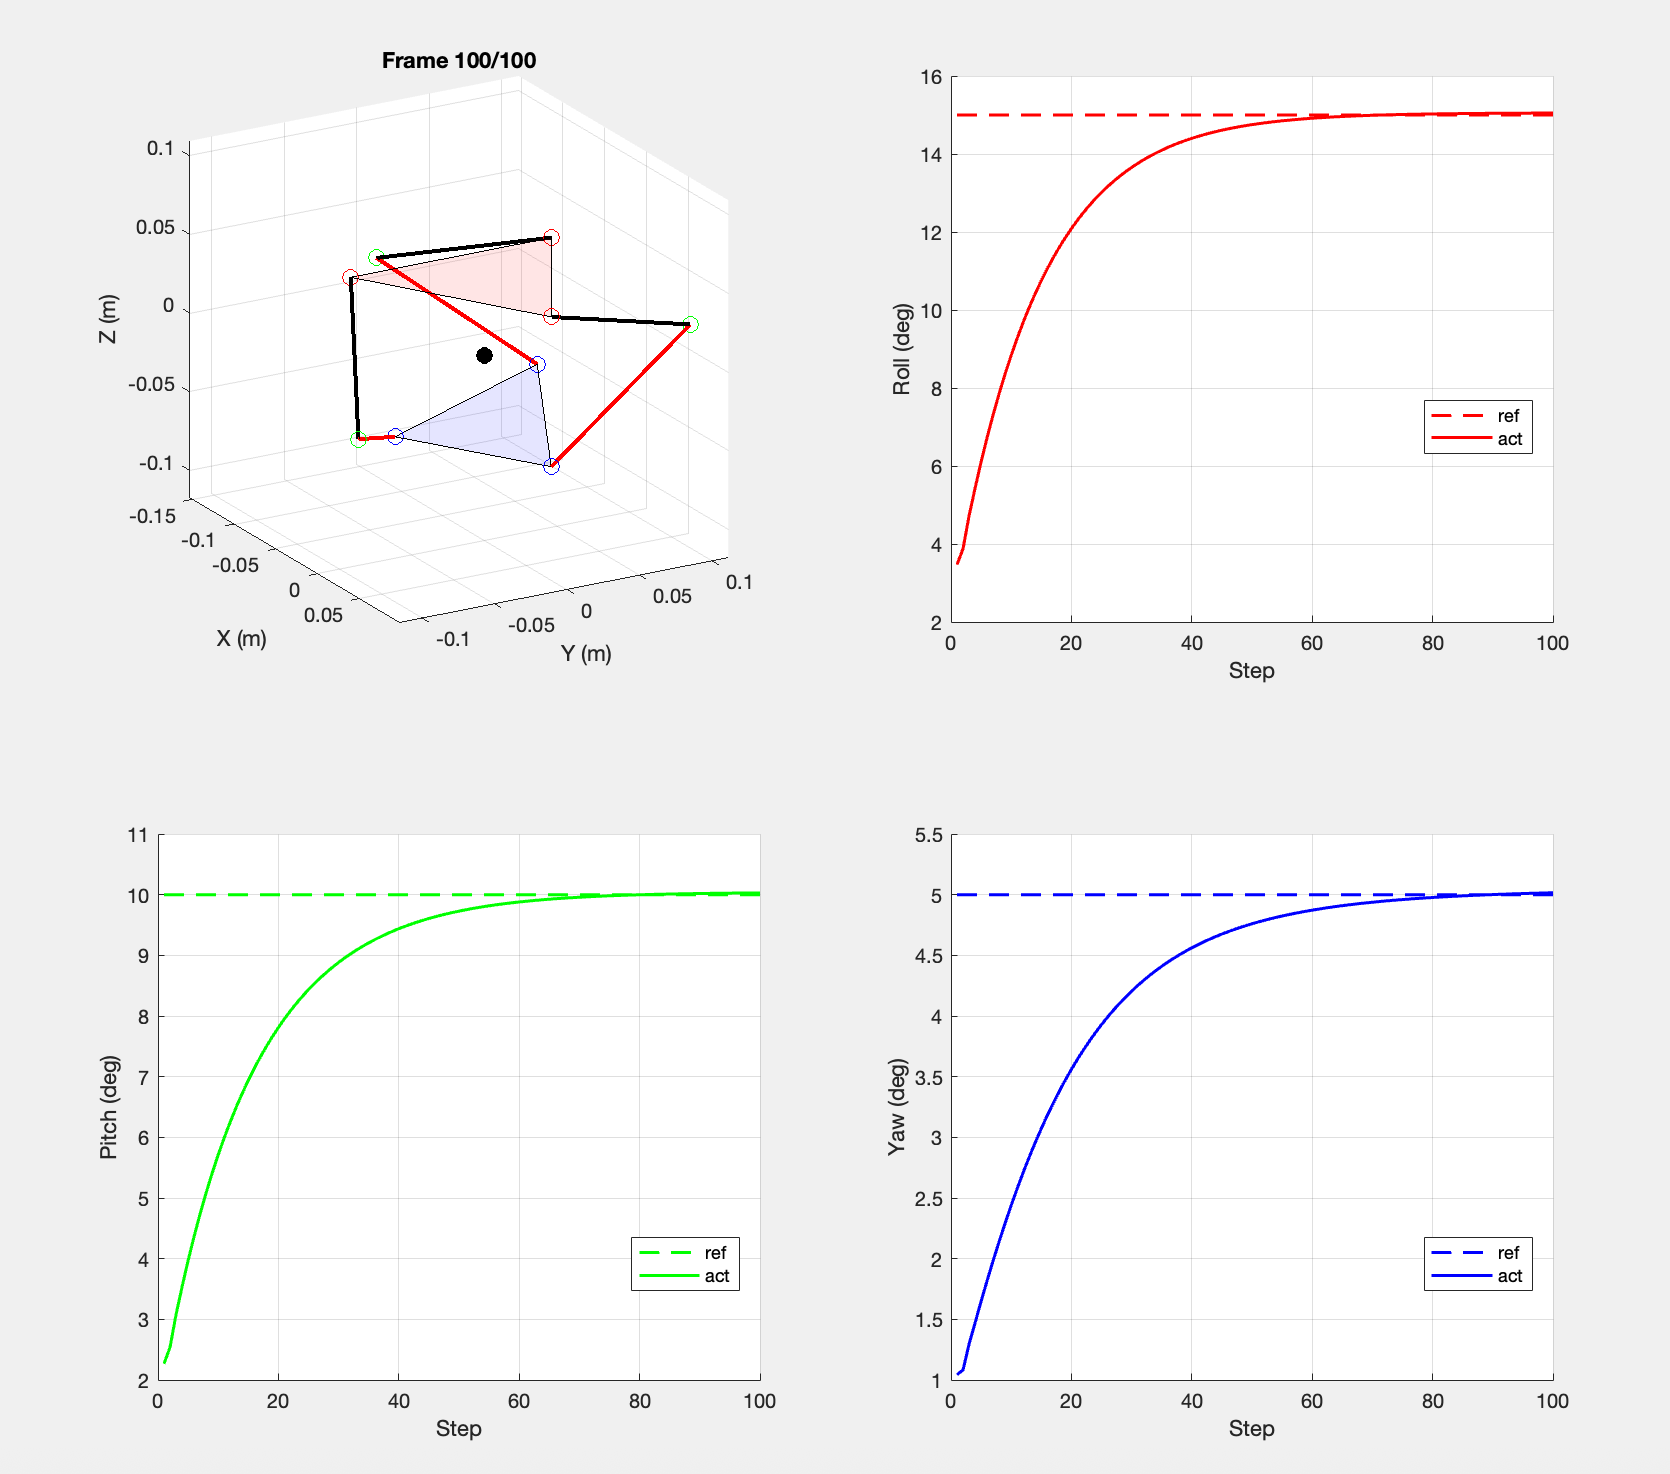
\includegraphics[width=\linewidth]{underdamped_response.png}
  \caption{Platform orientation (roll, pitch, yaw) under underdamped PID gains.  Compliance is high, yielding oscillatory settling.}
  \label{fig:underdamped}
\end{figure}



\subsection{Simulation Results}
Figures~\ref{fig:underdamped} and \ref{fig:critical} show the end‑effector orientation tracking under the two tuning sets for a step reference of \([15^\circ,\;10^\circ,\;5^\circ]^T\).  The underdamped controller (Fig.~\ref{fig:underdamped}) exhibits sustained oscillations around the target due to low damping, whereas the critically damped controller (Fig.~\ref{fig:critical}) converges monotonically without overshoot.

\begin{figure}[h]
  \centering
  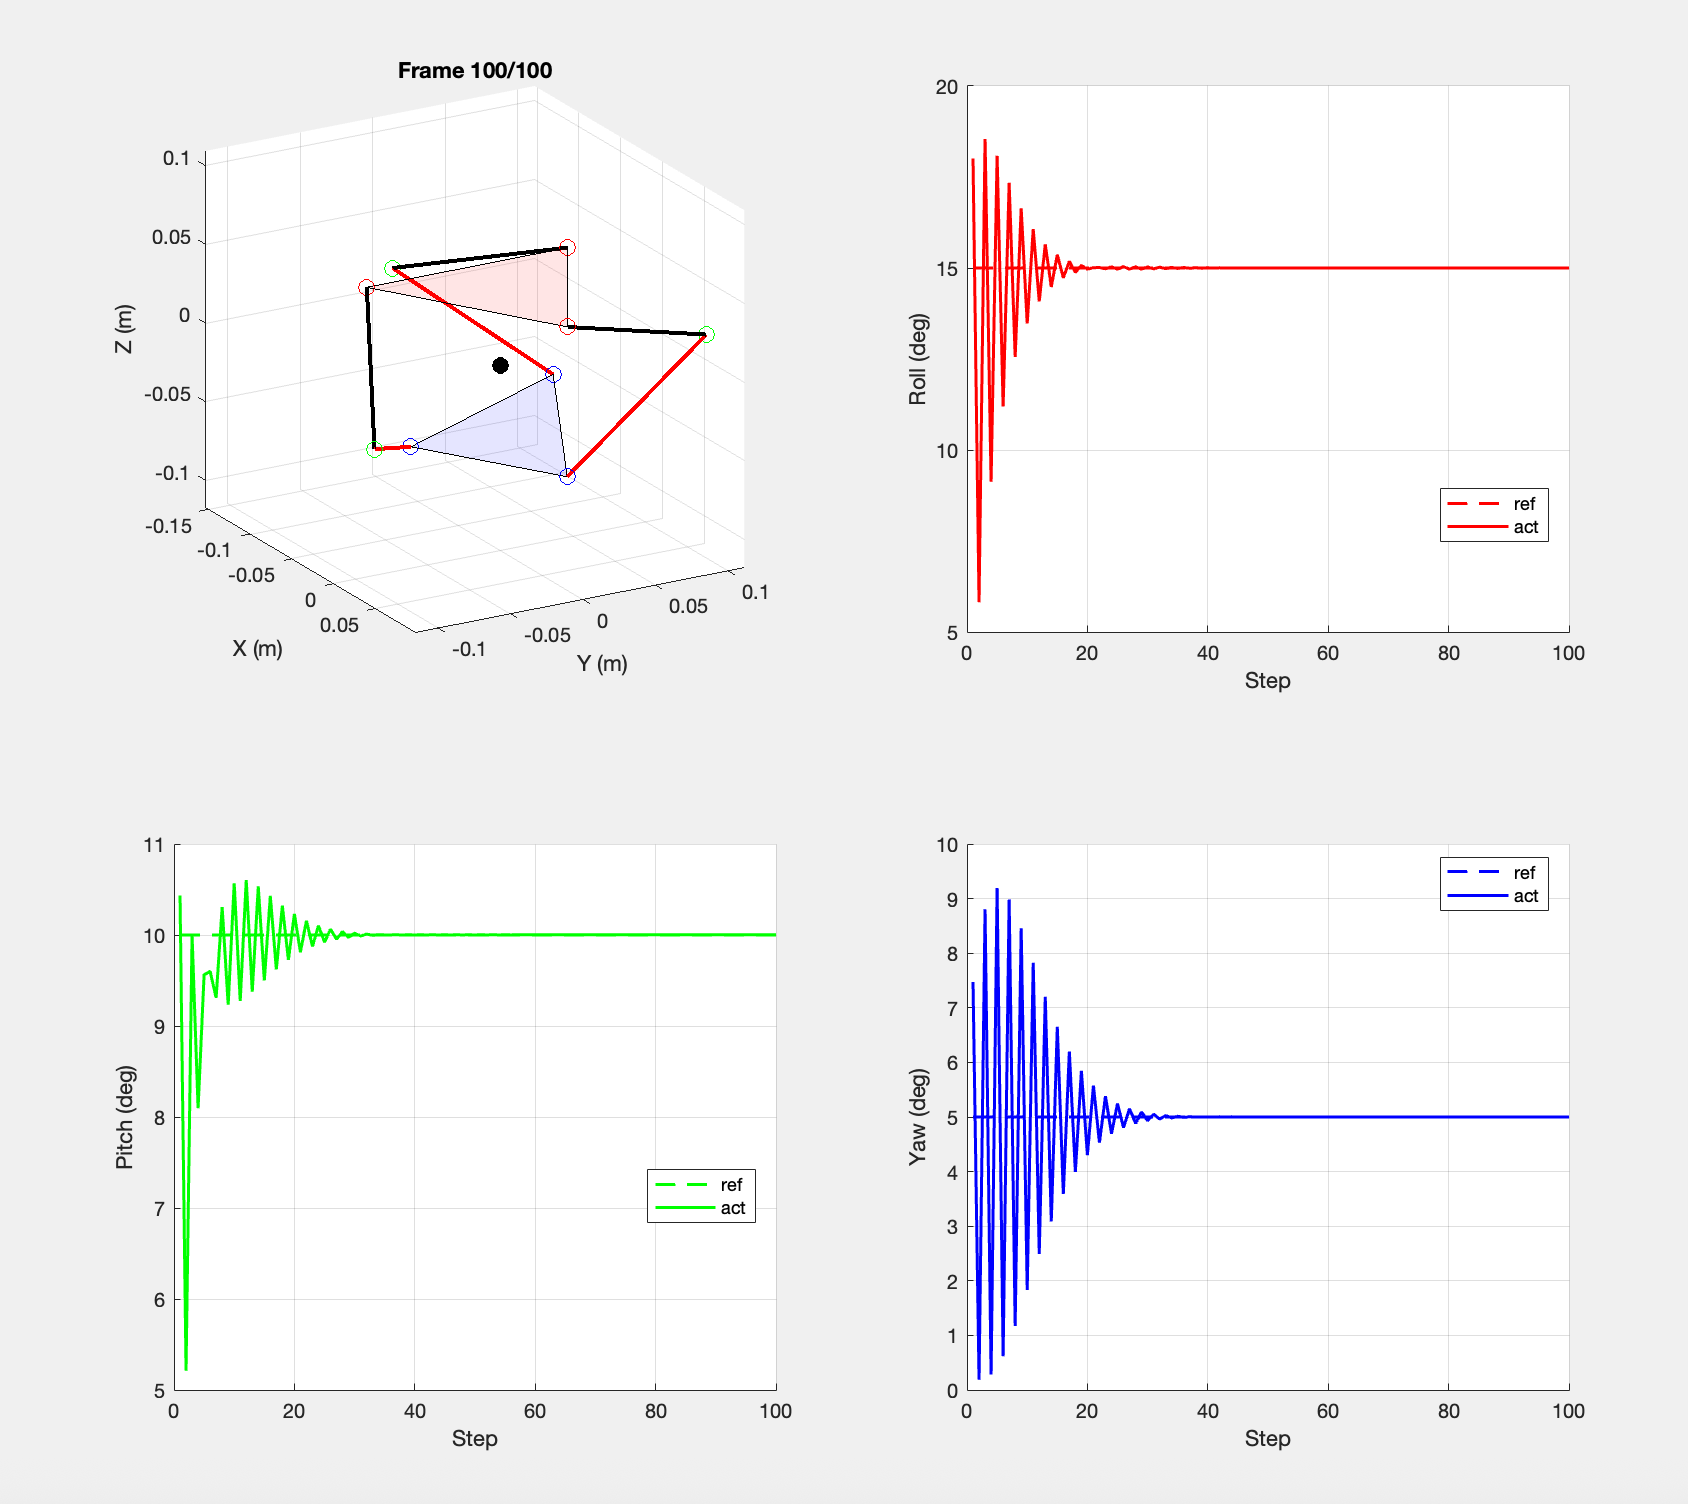
\includegraphics[width=\linewidth]{critical_response.png}
  \caption{Platform orientation under critically damped PID gains.  Compliance is low, yielding fast, non‑oscillatory convergence.}
  \label{fig:critical}
\end{figure}

\subsection{Discussion}
These results show that, although the 3‑RRR SPM is rigid, tuning feedback gains modulates its effective compliance: low‑stiffness settings allow larger deflections and oscillations for soft assistance, while high‑stiffness ensures precise, rapid tracking. Future work will add real‑time singularity monitoring—computing the Jacobian’s condition number to adjust gains or trigger avoidance maneuvers near singular poses—ensuring stable, safe operation across the workspace.

% \section{Broader Applications}

% % Originally designed for ankle rehabilitation, the 3-RRR spherical parallel mechanism (SPM) offers a versatile platform for human motion assistance and industrial applications.

% % In rehabilitation, it can be adapted into lower-limb exoskeletons\cite{exoskeleton_stroke} for patients with neurological disorders such as stroke, cerebral palsy, and spinal cord injuries. The mechanism's multi-DOF control allows for customized motion therapy, aiding in gait training, muscle recovery, and proprioception enhancement\cite{sale2012use}. It also has potential in sports rehabilitation, providing controlled resistance and guided movement to optimize recovery.

% % Beyond medical applications, the high stiffness and precision of the 3-RRR SPM make it ideal for industrial automation. It can enhance robotic arms for precise alignment, be miniaturized for robotic end-effectors, or be applied to adaptive fixturing in CNC machining\cite{bakker2013active}. The ability to execute controlled pitch, yaw, and roll enables efficient workpiece positioning, improving manufacturing accuracy and flexibility.

% Originally designed for ankle rehabilitation, the 3-RRR spherical parallel mechanism (SPM) is a versatile platform for human motion assistance and industrial applications.

% In rehabilitation, it can be integrated into lower-limb exoskeletons\cite{exoskeleton_stroke} for patients with neurological disorders like stroke and spinal cord injuries. Its multi-DOF control supports customized motion therapy, aiding in gait training, muscle recovery, and proprioception enhancement\cite{sale2012use}. It also holds potential in sports rehabilitation by providing controlled resistance and guided movement.

% Beyond medical applications, the 3-RRR SPM’s high stiffness and precision make it valuable for industrial automation. It can enhance robotic arms, be miniaturized for robotic end-effectors, or assist in adaptive fixturing for CNC machining\cite{bakker2013active}. Its controlled pitch, yaw, and roll improve workpiece positioning, enhancing manufacturing accuracy and flexibility.
\section{Conclusion and Future Work}

In summary, we introduced a compact, wearable 3‑RRR ankle rehabilitation robot and a complete design‑to‑dynamics workflow—from portable mechanical design to kinematic and dynamic modeling and simulation‑based control. Simulations and 3D‑printed prototype tests validated key ankle motions and demonstrated robust, compliance‑modulated performance across the workspace.

Building on these results, we are going to develop a self‑adaptive framework that fuses in‑shoe IMU and plantar‑pressure sensing with real‑to‑sim model personalization. A fuzzy‑logic impedance controller will operate around dynamically estimated joint axes and switch modes based on gait phase, enabling smooth transitions from static ROM training to gait‑timed assistance.

Earlier analyses assumed a single, concentric center of rotation; future design iterations will replace this with a dual‑axis, non‑concentric ankle model to better match human biomechanics and improve ergonomic comfort. Planned human‑subject studies will validate alignment, comfort and therapeutic efficacy.

Beyond clinical rehabilitation, this platform can be reconfigured as an assistive walking or running device for individuals with neuromuscular impairments, providing real‑time balance correction and dynamic support to enhance mobility and quality of life!

\section*{Acknowledge}

The authors would like to express their gratitude to Professor Sunil for his invaluable guidance and support throughout this project. We also appreciate the collaborative efforts of our team members in designing, modeling, and evaluating the proposed system.


\bibliographystyle{IEEEtran}  
% \bibliography{main}
\begin{thebibliography}{99}

\bibitem{gosselin1989optimum}
Gosselin, C. M., \& Angeles, J. (1989). The optimum kinematic design of a spherical three-degree-of-freedom parallel manipulator. \textit{Journal of Mechanisms, Transmissions, and Automation in Design}, 111(2), 202-207.

\bibitem{merlet2006parallel}
Merlet, J.-P. (2006). Jacobian, manipulability, condition number, and accuracy of parallel robots. \textit{The International Journal of Robotics Research}, 25(6), 557-571.

\bibitem{he2021spindle}
He, P., Kantu, N. T., Xu, B., Swami, C. P., Saleem, G. T., \& Kang, J. (2021). A novel 3-RRR spherical parallel instrument for daily living emulation (SPINDLE) for functional rehabilitation of patients with stroke. \textit{International Journal of Advanced Robotic Systems}, 18(3). \url{https://doi.org/10.1177/17298814211012325}

\bibitem{exoskeleton_stroke}
Dollar, A. M., \& Herr, H. (2008). Lower extremity exoskeletons and active orthoses: Challenges and state-of-the-art. \textit{IEEE Transactions on Robotics}, 24(1), 144-158.

\bibitem{sadeqi2017design}
Sadeqi, S., Bourgeois, S. P., Park, E. J., \& Arzanpour, S. (2017). Design and performance analysis of a 3-RRR spherical parallel manipulator for hip exoskeleton applications. \textit{Journal of Rehabilitation and Assistive Technologies Engineering}, 4, 2055668317697596. \url{10.1177/2055668317697596}

\bibitem{sale2012use}
Sale, P., Franceschini, M., Waldner, A., Hesse, S., et al. (2012). Use of the robot assisted gait therapy in rehabilitation of patients with stroke and spinal cord injury. \textit{European Journal of Physical and Rehabilitation Medicine}, 48(1), 111-121.

\bibitem{bakker2013active}
Bakker, O. J., Papastathis, T. N., Popov, A. A., \& Ratchev, S. M. (2013). Active fixturing: literature review and future research directions. \textit{International Journal of Production Research}, 51(11), 3171-3190.

\bibitem{wu2019design}
Wu, G., \& Bai, S. (2019). Design and kinematic analysis of a 3-RRR spherical parallel manipulator reconfigured with four-bar linkages. \textit{Robotics and Computer-Integrated Manufacturing}, 56, 55-65. \url{10.1016/j.rcim.2018.08.006}

\bibitem{dong2021state}
Dong, M., Zhou, Y., Li, J., Rong, X., Fan, W., Zhou, X., \& Kong, Y. (2021). State of the art in parallel ankle rehabilitation robot: a systematic review. \textit{Journal of NeuroEngineering and Rehabilitation}, 18(1). \url{10.1186/s12984-021-00845-z}

\bibitem{chai2014root}
Chai, T., \& Draxler, R. R. (2014). Root mean square error (RMSE) or mean absolute error (MAE). \textit{Geoscientific Model Development Discussions}, 7(1), 1525-1534.

\bibitem{james2024rehabilitation}
James, S. G. (1995). Rehabilitation of the foot and ankle. \textit{Online resource}. Available at: \url{https://cir.nii.ac.jp/crid/1130000793859809792}

\bibitem{brockett2016biomechanics}
Brockett, C. L., \& Chapman, G. J. (2016). Biomechanics of the ankle. \textit{Orthopaedics and Trauma}, 30(3), 232-238. \url{10.1016/j.mporth.2016.04.015}

\end{thebibliography}





\end{document}
